\task{Об одной задаче классификации}
\begin{itemize}

\itA Очевидно, что ширина этой полосы не может быть больше, чем расстояние между самыми близкими друг к другу точками кругов. Сделаем ширину полосы равной этому расстоянию.

Для этого соединим центры кругов отрезком и построим касательные к кругам в в точках пересечения отрезка с их границей. Они будут параллельны и образуют полосу максимально допустимой ширины (смотреть рисунок).

\begin{center}
	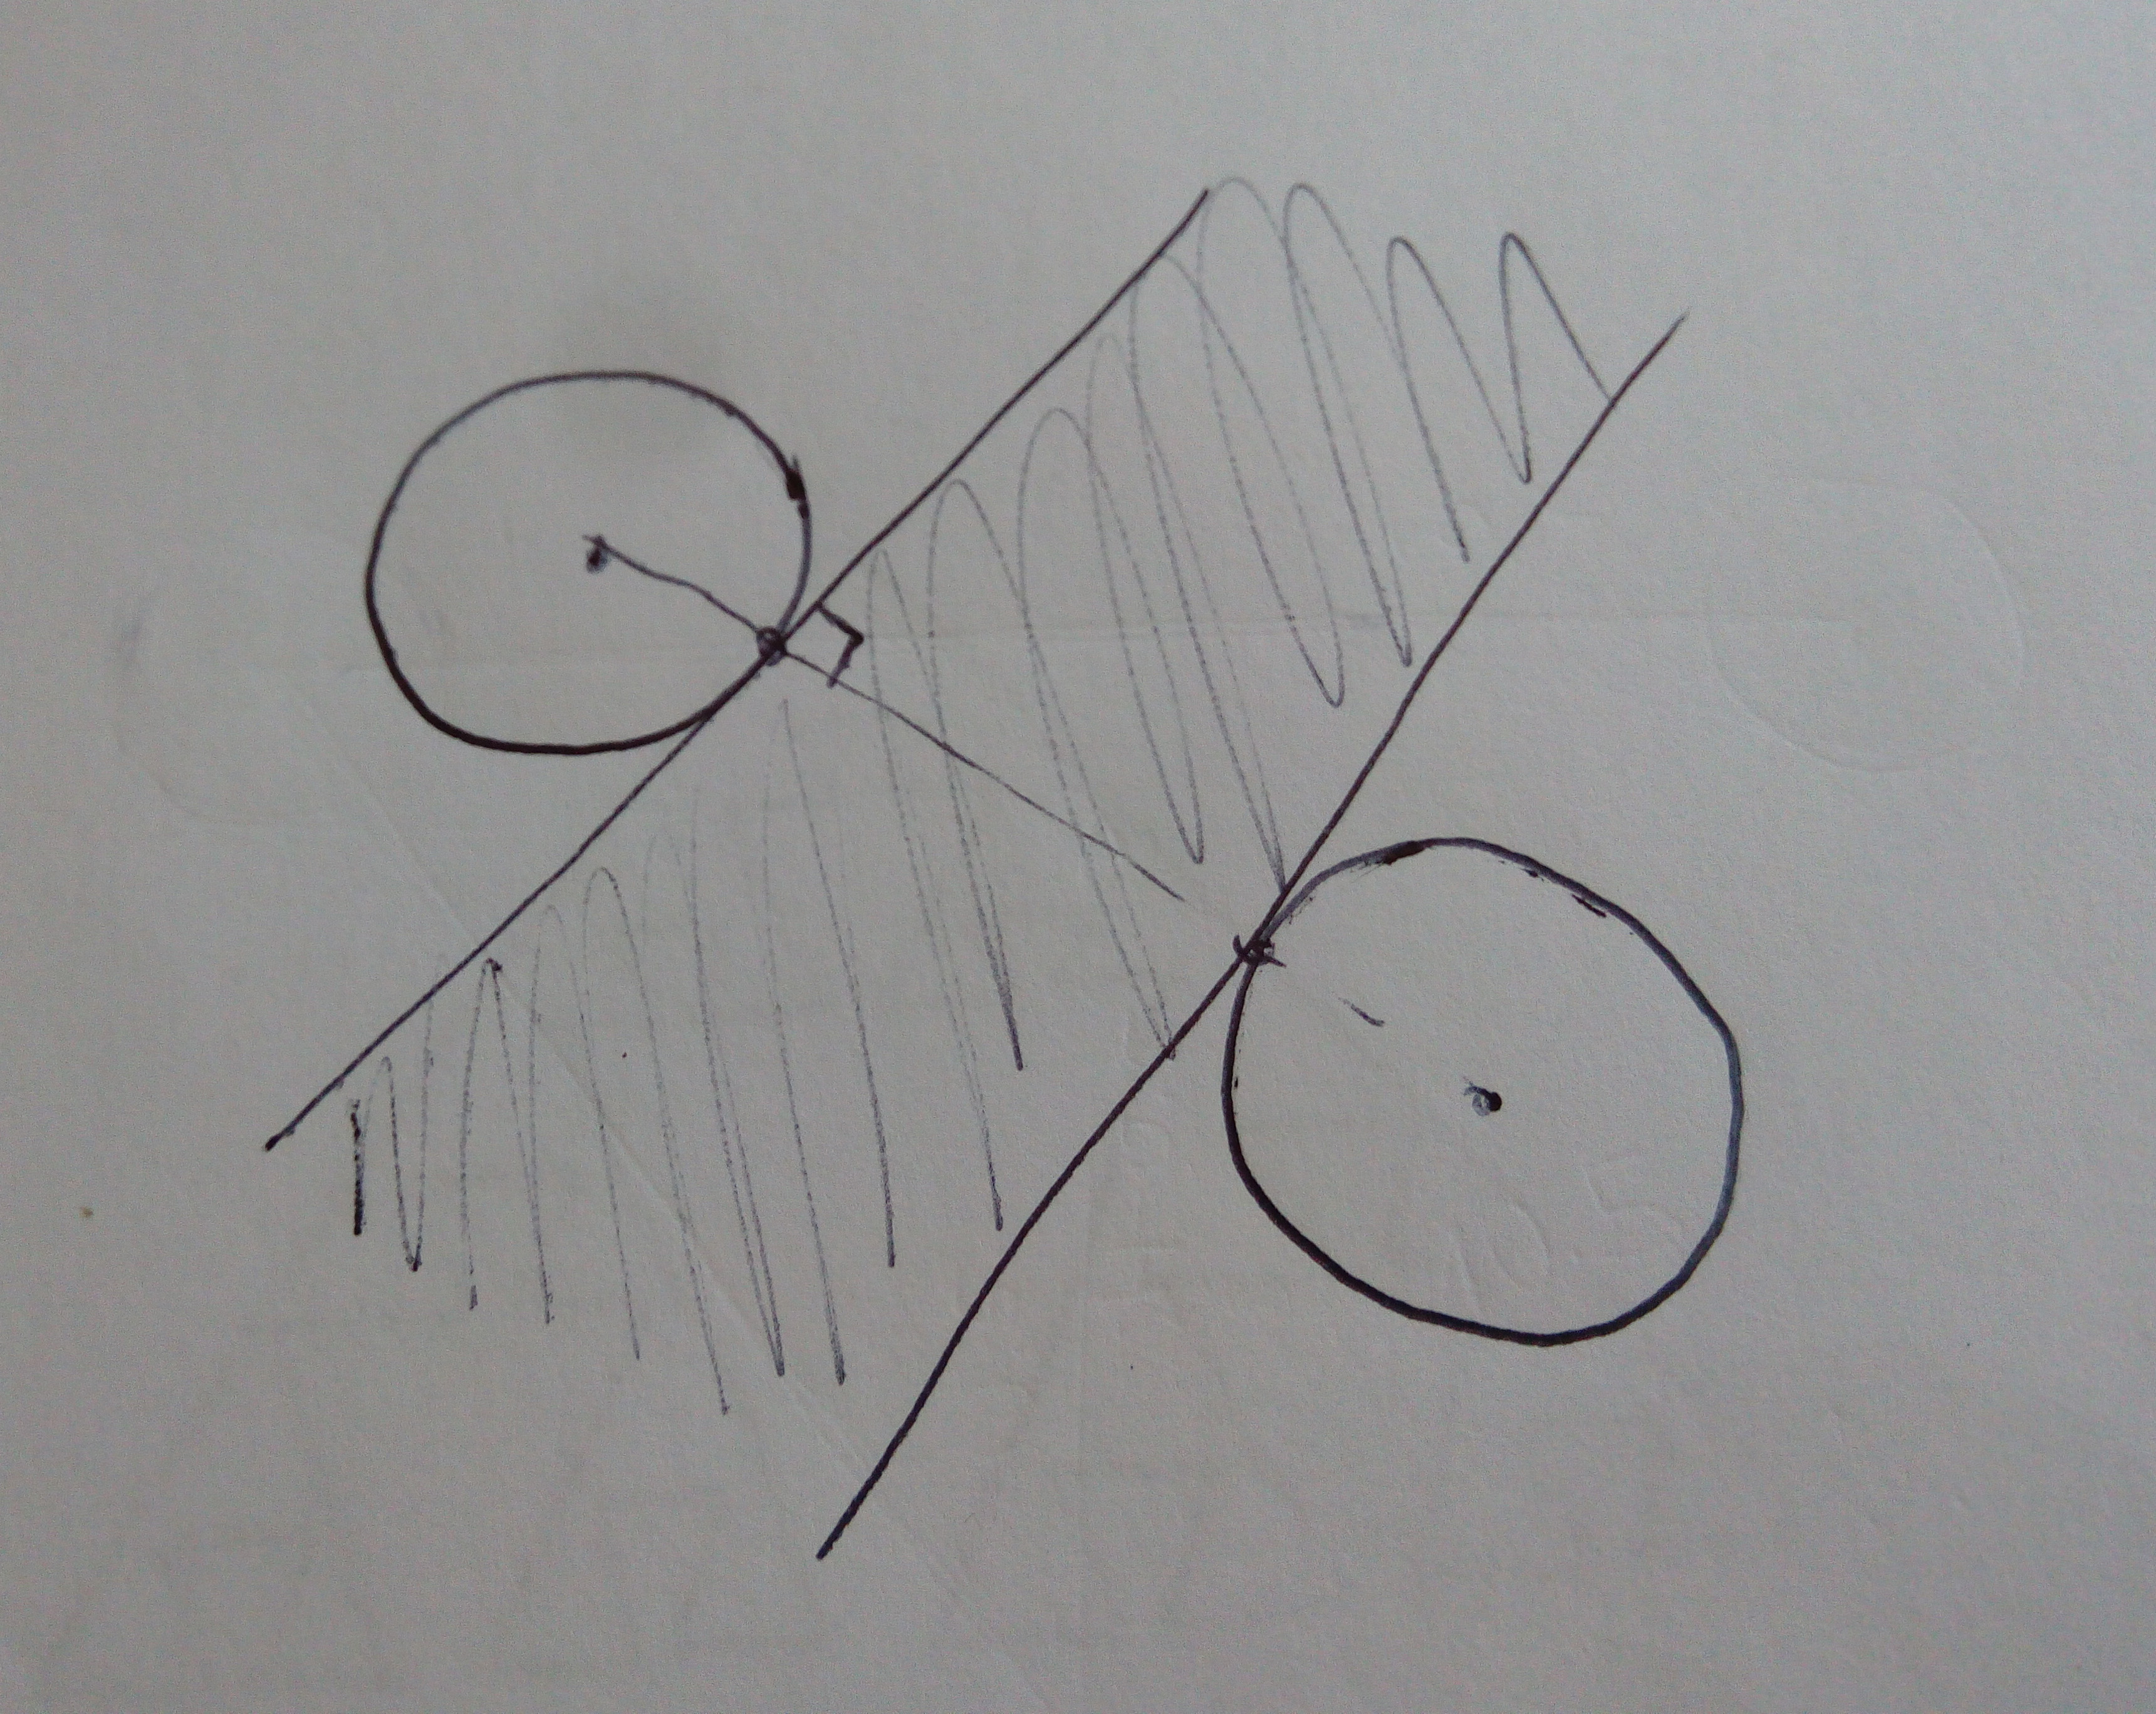
\includegraphics[natwidth=3441,natheight=2736,width=6cm]{figures/2018-simple-svm}
\end{center}

\item[\bf B.–C.] Сработает похожий метод: надо найти ближайшие друг к другу точки квадратов и соединить их отрезком — искомая полоса получится, если провести к данному отрезку перпендикуляры в его концах.

С одной стороны, её ширина будет максимально допустимой, потому что она будет равна расстоянию между ближайшими точками квадратов, а большая ширина запрещена.

С другой стороны, ни одна точка из квадратов не попадёт внутрь этой полосы, потому что квадрат — выпуклый многоугольник. В силу этого он либо лежит по одну сторону от прямой, проходящей через точку его границы, либо лежит по обе стороны, и с каждой из сторон от прямой находится часть стороны, на которой лежала точка, через которую мы проводили прямую.

Но тогда на части этой стороны, лежащей внутри полосы, найдётся точка, которая ближе к другому концу отрезка, лежащем на другом краю полосы, что противоречит построению полосы.
\end{itemize}